\begin{figure*}[t]
  \center
  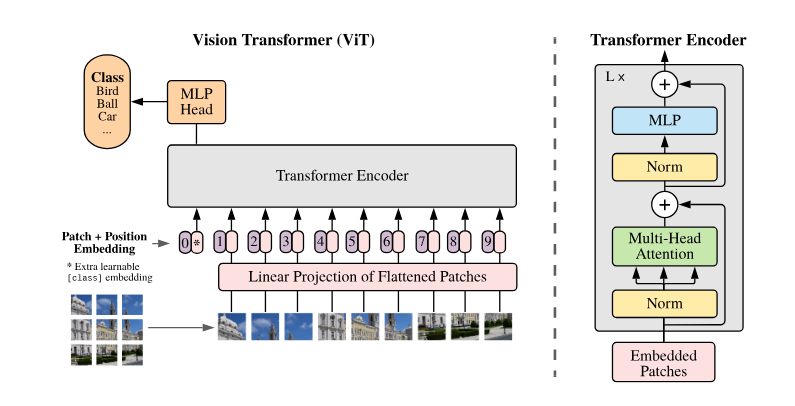
\includegraphics[width=1\textwidth]{images/vit-architecture.png}
  \caption{The Vision Transformer (ViT) architecture from \cite{alexey2020image}. On the left the model architecture while on the right the Transformer encoder block architecture from \cite{vaswani2017attention}.}
  \label{fig:vit-architecture}
\end{figure*}

\section{Architecture}

In recent years, the Transformer architecture originally developed for Natural Language Processing has been successfully applied to Computer Vision tasks. The Vision Transformer (ViT) rethinks image classification by treating an image as a sequence of patches, much like tokens in a sentence, and processes them using standard Transformer blocks. In this chapter, we detail the architecture of the Vision Transformer and provide the mathematical foundations underlying its design.

\subsection{Overview}
The Vision Transformer (ViT) adapts the Transformer architecture originally developed for Natural Language Processing to image classification tasks. Instead of processing an image as a whole, ViT divides it into a sequence of patches (analogous to tokens) and processes these patches through a stack of Transformer encoder blocks. The key steps in the ViT pipeline are:

\begin{enumerate}
  \item \textbf{Patch Embedding}: The input image is divided into fixed size patches that are flattened and projected into a latent space.
  \item \textbf{Positional Encoding}: Since Transformers are permutation invariant, positional embeddings are added to the patch embeddings.
  \item \textbf{Transformer Encoder}: A series of Transformer encoder blocks processes the sequence of embeddings using self attention and feed forward networks.
  \item \textbf{Classification Head}: The encoder output is used by a classification head for the final prediction.
\end{enumerate}

\subsection{Patch Embedding}

\textbf{Patch Extraction}

Given an input image
\begin{equation}
  \mathbf{X} \in \mathbb{R}^{H \times W \times C}
\end{equation}
where \(H\) and \(W\) denote the height and width of the image, and \(C\) denotes the number of channels, the image is divided into \(N\) patches of size \(P \times P\). Hence, the number of patches is:
\begin{equation}
  N = \frac{HW}{P^2}
\end{equation}

\textbf{Flattening and Linear Projection}

Each patch, denoted as \(\mathbf{x}_p \in \mathbb{R}^{P \times P \times C}\), is flattened into a vector of dimension \(P^2 \cdot C\). A learnable linear projection (implemented as a fully connected layer) maps this vector into a \(D\)-dimensional embedding space:

\begin{equation}
  \mathbf{z}_p = \mathbf{W}_e \mathbf{x}_p + \mathbf{b}_e
\end{equation}

where $\mathbf{W}_e \in \mathbb{R}^{D \times (P^2 \cdot C)} \text{ and } \mathbf{b}_e \in \mathbb{R}^{D}$.

After processing all patches, we obtain a sequence of embeddings:

\begin{equation}
  \mathbf{Z} = \left[\mathbf{z}_1, \mathbf{z}_2, \dots, \mathbf{z}_N\right] \in \mathbb{R}^{N \times D}
\end{equation}

%%%%%%%%%%%%%%%%%%%%%%%%%%%%%%%%%%%%%%%%%%%%%%%%%%
\subsection{Positional Encoding}

Transformers do not inherently capture the order or spatial structure of input data. To inject spatial information, learnable positional embeddings are added to the patch embeddings. Let:
\begin{equation}
  \mathbf{E}_{\text{pos}} \in \mathbb{R}^{N \times D}
\end{equation}

be a set of positional embeddings. The combined input to the Transformer encoder is then:
\begin{equation}
  \mathbf{Z}_0 = \mathbf{Z} + \mathbf{E}_{\text{pos}}
\end{equation}

In some implementations, a special class token \(\mathbf{z}_{\text{cls}} \in \mathbb{R}^{D}\) is prepended to the sequence:
\begin{equation}
  \mathbf{Z}_0 = \left[\mathbf{z}_{\text{cls}}, \mathbf{z}_1, \dots, \mathbf{z}_N \right]
\end{equation}

%%%%%%%%%%%%%%%%%%%%%%%%%%%%%%%%%%%%%%%%%%%%%%%%%%
\subsection{Transformer Encoder}

The Vision Transformer uses a stack of \(L\) Transformer encoder blocks. Each block is composed of two main components: the Multi-Head Self-Attention (MHSA) mechanism and a Feed-Forward Network (FFN). Layer normalization (LN) and residual connections are applied around each component.

\textbf{Multi-Head Self-Attention (MHSA)}

Let \(\mathbf{Z}^{(l-1)} \in \mathbb{R}^{M \times D}\) be the input to the \(l\)-th encoder block, where \(M\) is the number of tokens (including the class token if used).

\textbf{Query, Key, and Value}

The input is projected into query (\(\mathbf{Q}\)), key (\(\mathbf{K}\)), and value (\(\mathbf{V}\)) matrices using learnable projection matrices \(\mathbf{W}_Q, \mathbf{W}_K, \mathbf{W}_V \in \mathbb{R}^{D \times D}\):

\begin{itemize}
  \item \(\mathbf{Q} = \mathbf{Z}^{(l-1)} \mathbf{W}_Q\)
  \item \(\mathbf{K} = \mathbf{Z}^{(l-1)} \mathbf{W}_K\)
  \item \(\mathbf{V} = \mathbf{Z}^{(l-1)} \mathbf{W}_V\)
\end{itemize}

For multi-head attention, these are divided into \(h\) heads. For head \(i\) (\(i=1,\dots,h\)), we have:
\begin{equation}
  \mathbf{Q}_i, \mathbf{K}_i, \mathbf{V}_i \in \mathbb{R}^{M \times d} 
\end{equation}

with $d = \frac{D}{h}$.

\textbf{Scaled Dot-Product Attention}

For head \(i\), the attention is computed as:
\begin{equation}
  \text{Att}_i(\mathbf{Q}_i, \mathbf{K}_i, \mathbf{V}_i) = \text{softmax}\left(\frac{\mathbf{Q}_i \mathbf{K}_i^\top}{\sqrt{d}}\right) \mathbf{V}_i
\end{equation}

The scaling by \(\sqrt{d}\) ensures numerical stability.

\textbf{Concatenation and Final Projection}

The outputs from all \(h\) heads are concatenated and projected:
\begin{equation}
    \text{MHSA}(\mathbf{Q}, \mathbf{K}, \mathbf{V}) = \text{Concat}\left(\text{Att}_1, \dots, \text{Att}_h\right) \mathbf{W}_O
    \label{eq:mhsa}
\end{equation}

with \(\mathbf{W}_O \in \mathbb{R}^{D \times D}\) being a learned projection matrix.

\textbf{Residual Connection and Normalization}

A residual connection and layer normalization are applied:

\begin{equation}
\mathbf{Z}^{\prime(l)} = \text{LN}\left(\mathbf{Z}^{(l-1)} + \text{MHSA}(\mathbf{Q}, \mathbf{K}, \mathbf{V})\right)
\label{eq:residual}
\end{equation}

\textbf{Feed-Forward Network (FFN)}

Each encoder block contains a two-layer FFN applied to each token independently:

\begin{equation}
  \text{FFN}(\mathbf{z}) = \text{GELU}\left(\mathbf{z} \mathbf{W}_1 + \mathbf{b}_1\right) \mathbf{W}_2 + \mathbf{b}_2,
\end{equation}

where:
\begin{itemize}
  \item \(\mathbf{W}_1 \in \mathbb{R}^{D \times D_{\text{ff}}}\)
  \item \(\mathbf{W}_2 \in \mathbb{R}^{D_{\text{ff}} \times D}\)
  \item \(D_{\text{ff}}\) is the dimension of the hidden layer
  \item GELU is the Gaussian Error Linear Unit activation
\end{itemize}

A residual connection and layer normalization follow:
\begin{equation}
  \mathbf{Z}^{(l)} = \text{LN}\left(\mathbf{Z}^{\prime(l)} + \text{FFN}(\mathbf{Z}^{\prime(l)})\right)
\end{equation}

%%%%%%%%%%%%%%%%%%%%%%%%%%%%%%%%%%%%%%%%%%%%%%%%%%
\subsection{Classification Head}

For classification tasks, the output corresponding to the class token is used. For instance, if a class token \(\mathbf{z}_{\text{cls}}\) is used, the final prediction is obtained as:

\begin{equation}
  \hat{y} = \text{softmax}\left(\mathbf{W}_c \mathbf{z}_{\text{cls}} + \mathbf{b}_c\right)
\end{equation}

where \(\mathbf{W}_c \in \mathbb{R}^{K \times D}\) and \(\mathbf{b}_c \in \mathbb{R}^{K}\) are the weights and bias of the classification layer, and \(K\) is the number of classes. Alternatively, a global average pooling can be applied to the token embeddings before the linear projection.

%%%%%%%%%%%%%%%%%%%%%%%%%%%%%%%%%%%%%%%%%%%%%%%%%%

\section{Differences from Convolutional Neural Networks}
The differences between Convolutional Neural Networks (CNNs) architecture in Figure \ref{fig:cnn-arch} and Vision Transformers (ViTs) come from their architectural philosophies and how they process visual data. CNNs rely on convolutional layers with localized receptive fields, using spatial hierarchies (kernels and pooling) to progressively extract features. These layers prioritize local spatial relationships and translation invariance, making CNNs data efficient for smaller datasets. In contrast, Vision Transformers treat images as sequences of flattened patches, leveraging self attention mechanisms to model global interactions between all patches from the first layer. This allows ViTs to capture long range dependencies directly but often requires large scale training data to generalize effectively, as they lack the inductive biases (locality) typical to CNNs. Additionally, ViTs replace spatial hierarchies with a uniform processing of patch tokens across all layers, while CNNs gradually reduce spatial resolution while expanding channel depth.

\begin{figure}[H]
    \centering
    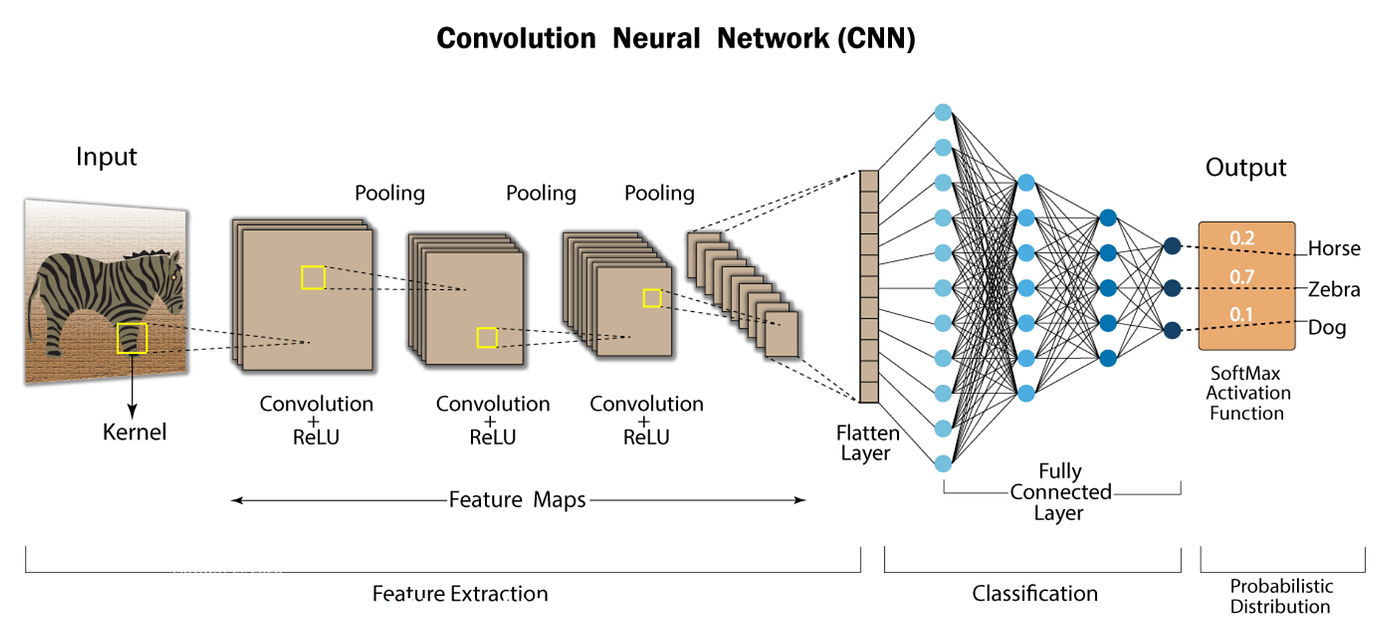
\includegraphics[width=0.5\textwidth]{images/cnn_architecture.png}
    \caption{A typical Convolutional Neural Network (CNN) architecture with convolutional and pooling layers.}
    \label{fig:cnn-arch}
\end{figure}